\documentclass[tikz]{standalone}


\usepackage{xcolor}
\usetikzlibrary{matrix, positioning, shapes, fit}

\begin{document}
    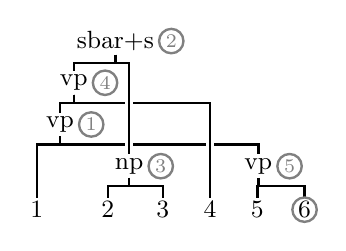
\begin{tikzpicture}[
        edge from parent path={(\tikzparentnode.south) -- ++(0,-.7ex) -| (\tikzchildnode.north)},
        every path/.style={line width=.2ex},
        level distance=3.5ex,
        node distance=0ex,
        anchor=center,
        level 1/.style={sibling distance=8em},
        level 2/.style={sibling distance=5em},
        level 3/.style={sibling distance=4em},
        every node/.style={font=\small}
        ]
%        \matrix (pos) [matrix of nodes, every node/.style={anchor=center, inner sep=0pt}, column sep=4ex] {
%             ~ & ~ & ~ & ~ & ~ & ~ \\
%        };
        \coordinate (pos-1-1) at (0,0);
        \coordinate (pos-1-2) at (.9,0);
        \coordinate (pos-1-3) at (1.6,0);
        \coordinate (pos-1-4) at (2.2,0);
        \coordinate (pos-1-5) at (2.8,0);
        \coordinate (pos-1-6) at (3.4,0);
        \coordinate[fit=(pos-1-1)(pos-1-6)] (pos) {};

        \begin{scope}[every node/.style={font=\small, inner sep=1pt}]
            \node[above=14ex of pos, xshift=-2em] (sbar) {\cn{sbar}+\cn{s}}
            child { node[xshift=2.5em] (vp1) {\cn{vp}}
                child { node[xshift=2em] (vp2) {\cn{vp}}
                    child { node[above= of pos-1-1] {1} }
                    child { node[xshift=12ex] (vpbin) {\cn{vp}\binsym{}}
                        child { node[above=of pos-1-5] (term4) {5} }
                        child { node[above=of pos-1-6] (prt) {6}   }}}
                child {
                    node[above=of pos-1-4] (term3) {4}}}
            child { node[yshift=-7ex, xshift=-3.5em] (np) {\cn{np}}
                child { node[above=of pos-1-2] (term1) {2} }
                child {
                    node[above=of pos-1-3] (term2) {3}}};
        \end{scope}

        % shortest guide
        \begin{scope}[font=\small, gray, every node/.style={inner sep=1pt, circle, draw, font=\scriptsize}]
            \node [right=of sbar] {2};
            \node [right=of np] {3};
            \node [right=of vp1] {4};
            \node [right=of vp2] {1};
            \node [right=of vpbin] {5};
            \node[draw, gray, circle] at (prt) {\phantom{1}};
        \end{scope}

        % redraw corssing edges with white foundation
        \begin{scope}
            \draw[white, line width=.7ex] (vp1.south) -- ++(0,-.7ex) -| (term3.north);
            \draw (vp1.south) -- ++(0,-.7ex) -| (vp2.north);
            \draw (vp1.south) -- ++(0,-.7ex) -| (term3.north);

            \draw[white, line width=.7ex] (sbar.south) ++(.5pt,-.5ex) -| (np.north);
            \draw (sbar.south) -- ++(0,-.7ex) -| (np.north);
            \draw (sbar.south) -- ++(0,-.7ex) -| (vp1.north);
        \end{scope}
    \end{tikzpicture}
\end{document}
